%%%%%%%%%%%%%%%%%%%%%%%%%%%%%%%%%%%%%%%%%%%%%%%%%%%%%%%%%%%%%%%%%%%%%
% ========= CONFIGURATION DOCUMENT FOR COLLEGE REPORT (CS) =========%
%%%%%%%%%%%%%%%%%%%%%%%%%%%%%%%%%%%%%%%%%%%%%%%%%%%%%%%%%%%%%%%%%%%%%

\documentclass[
    12pt,                % Readable font dimention
    a4paper,             % Page format
    oneside,             % Print just front (change in 'twoside' for front-back)
    titlepage,           % Separate titlepage
    english              % Main language (for KOMA-Script)
]{report}              % 'scrreprt' is the 'report' class of KOMA-Script (more modern)

% --- 1. Fondamental packages (Format & language) ---
\usepackage[utf8]{inputenc}    % Input format for accented characters
\usepackage[T1]{fontenc}       % Output font format (better syllabation)
\usepackage[english]{babel}    % English manager
\usepackage{csquotes}          % Necessary for 'biblatex' for right quotes
\usepackage{float}
\usepackage[table]{xcolor}
% --- 2. Tipography & Layout ("Look & Feel") ---
\usepackage{lmodern}           % Use "Latin Modern" (enhanced version of the standard one)
\usepackage{microtype}         % Enhanced micro-tipography (giustification, spacing)
\usepackage[
    a4paper,
    margin=2.5cm               % Good margin, not eccessive
]{geometry}
\usepackage{setspace}          % Manage interline
\onehalfspacing                % Interline 1.5 (universitary report standard)

% --- 3. Color & Graphic ---
\usepackage{graphicx}                        % For include images
\usepackage{subcaption}
\usepackage{caption}
\usepackage[dvipsnames, table]{xcolor}       % For define and use colors
\definecolor{UniOrange}{rgb}{0.8, 0.4, 0.1}  % Average brite orange
\definecolor{UniBlue}{rgb}{0.1, 0.3, 0.7}    % Dark blue professional
\definecolor{DeepBlue}{rgb}{0, 0.2, 0.4}     % Very dark blue
\definecolor{LinkBlue}{rgb}{0.1,0.2,0.9}     % More brite blue

% --- 4. Header & Footer ---
\usepackage{fancyhdr}                        % Package to personalize header/footer
\pagestyle{fancy}
% Ensure enough head height for fancyhdr (suggested by package)
\setlength{\headheight}{14.49998pt}
\fancyhf{}                                   % Clean all fields
\fancyhead[L]{\nouppercase{\leftmark}}       % Chapter/section name to left
\fancyfoot[C]{\thepage}                      % Page number at center
\renewcommand{\headrulewidth}{0.4pt}         % Thin separation line
\renewcommand{\footrulewidth}{0pt}           % No footer line
\fancypagestyle{plain}{                      % 'Plain' page style (initial chapter)
    \fancyhf{}                               % Clean
    \fancyfoot[C]{\thepage}                  % Just page number
}

% --- 5. Title structure (Custumize Aesthetic) ---
\usepackage{titlesec}                            % Personalize title
\titleformat{\chapter}
    {\normalfont\huge\bfseries\color{UniOrange}} % Format
    {\thechapter.}                               % Number
    {10pt}                                       % Space
    {}                                           % Title
\titleformat{\section}
    {\normalfont\Large\bfseries\color{UniBlue}}
    {\thesection.}
    {8pt}
    {}
\titleformat{\subsection}
    {\normalfont\large\bfseries\color{DeepBlue}}
    {\thesubsection.}
    {8pt}
    {}

% --- 6. Useful packeges (Math & Code) ---
\usepackage{amsmath, amssymb, amsfonts} % Fondamentals for Math
\usepackage{booktabs}                   % Professional tables (use \toprule, \midrule,\bottomrule)
\usepackage{listings}
\usepackage{tcolorbox}

\tcbuselibrary{listings}

% --- 7. 'listings' style ---
\lstdefinestyle{mystyle}{
    commentstyle=\color{Green},
    keywordstyle=\color{LinkBlue}\bfseries,
    stringstyle=\color{red!80!black},
    numberstyle=\tiny\color{gray},
    basicstyle=\ttfamily\small,
    breakatwhitespace=false,
    breaklines=true,
    keepspaces=true,
    numbers=none,
    numbersep=5pt,
    showspaces=false,
    showstringspaces=false,
    showtabs=false,
    tabsize=2,
}

% Specific for code in bash
\lstdefinestyle{bashstyle}{
    style=mystyle,    
    language=bash,    
    morekeywords={    
        rm, ssh, scp, ls, cd, grep, apt, get, yum, systemctl,
        mv, cp, mkdir, chmod, chown, cat, nano, vim, service, shutdown, ip, netplan, ln, systemctl, restart, VBoxManage, mpirun, touch, docker, hpcc, stress, ng, sysbench, iperf3, iozone
    }
}

% --- 8. Code box smoother & prettier ---
\newtcblisting[auto counter]{codice}[2][]{
    arc=3mm,
    colback=orange!5,
    colframe=orange!80,
    boxrule=0.8pt,
    % ----- Title Options -----
    title={Code \thetcbcounter: #2},
    colbacktitle=DeepBlue,
    coltitle=white,
    fonttitle=\bfseries,
    % ----- LISTINGS Options -----
    listing only,
    listing options={
        style=mystyle, 
        #1
    }
}

% --- 7. Bibliography ---
\usepackage[
    backend=biber,     % Engine to manage bibliography (modern)
    style=ieee,        % Common style in CS (numeric)
    sorting=none       % Order for citation
]{biblatex}
\addbibresource{bibliography.bib} % .bib file name

% --- 8. Link e Quotes ---
\usepackage{hyperref}
\hypersetup{
    colorlinks=true,
    linkcolor=LinkBlue,           % Internal link color
    citecolor=OliveGreen,         % Citations color
    urlcolor=LinkBlue             % External link color (URL)
}

% --- Metadati per la Pagina del Titolo ---

\title{
    \centering
    
\includegraphics[width=6cm]{settings/units_blue_logo.png}
    \par
    \vspace{0.5cm} % Spazio tra logo e titolo
    {\fontsize{45pt}{53pt}\selectfont
     \sffamily
     \bfseries
     \color{UniBlue}
     Performance Report
    }
    \\
    \vspace{0.2cm}
    {\fontsize{34pt}{38pt}\selectfont
     \sffamily
     \bfseries
     \color{UniBlue}
     Cloud Computing
    }
}
\author{
    \textbf{\color{UniOrange}Gabriele Granzotto} \\ 
    \textit{Università degli studi di Trieste} \\ 
    \texttt{\color{LinkBlue}gabriele.granzotto@studenti.units.it}
}
%%%%%%%%%%%%%%%%%%%%%%%%%%%%%%%%%%%%%%%%%%%%%%%%%%%%%%%%%%%%%%%%%%%%%%%%%%
% ========================= DOCUMENT BEGINNING ==========================%
%%%%%%%%%%%%%%%%%%%%%%%%%%%%%%%%%%%%%%%%%%%%%%%%%%%%%%%%%%%%%%%%%%%%%%%%%%
\begin{document}
% --- Pagina del Titolo ---
\maketitle % Crea la pagina del titolo
% --- Indice ---
\tableofcontents
\clearpage

% --- Capitoli del Report ---
\chapter{Introduction}

In the modern computer science industry, Software as a Service (SaaS) products and web applications are becoming increasingly important. \\
To fulfill this need, the industry creates tools to make developers' jobs easier and improve the scalability factor at the same time. \\
These two tools are:

\begin{itemize}
    \item Virtual Machines
    \item Containers
\end{itemize}

\thispagestyle{fancy}

\section{Tasks and Goals}
The goal of this report is to implement a cluster of Virtual Machines and a cluster of Containers. \\
Then I have to evaluate and compare the performance in computational power, memory, disk and network speed between the two infrastructures.

\section{Report Structure}
The program that I use to implement the virtual machine is VirtualBox. Instead, for the container, I use Docker. \\
The report will be structured into three parts:

\begin{itemize}
    \item a VMs setup section;
    \item a Containers setup section;
    \item the analysis of all the tests I make.
\end{itemize}

\chapter{Virtual Machines Setup}

Virtual Machines (VMs) are essential components of modern infrastructure, enabling multiple operating systems to run concurrently on a single physical host. This report analyzes the critical performance metrics of these virtualized environments.

\section{Create the VM}

I decide to use Oracle VirtualBox as a VM program. The reasons are that it is one of the most popular VM programs and most supported too. Nevertheless, it accurately represents the performance of that category of program.

\subsection{set VirtualBox}
The process of creating of a VM is quite easy, the entire process is done via a GUI:

\begin{itemize}
    \item press \textit{New} button;
    \item insert \textit{Name} of the VM and upload the ISO file of the chosen OS;
    \item choose CPU, RAM and DISK usage for the VM.
\end{itemize}

I choose to create a VM with 2 Core of CPU, 2GB of RAM and 25GB of virtual disk. \\
I think it is important to list the host machine specifications, to better interpret the results of tests that will follow.

\begin{table}[H]
    \centering
    \begin{tabular}{r|l}
        \color{UniOrange}{CPU}:  & Intel Core i5-8365U 1.60GHz \\
        \color{UniOrange}{RAM}:  & 16GB DDR4                   \\
        \color{UniOrange}{DISK}: & 256GB SSD NVMe
    \end{tabular}
    \caption{Hardware Specification}
    \label{tab:hardware}
\end{table}

\subsection{install the OS}

As Operative System, I choose to install \textbf{Ubuntu Server 24.04}. The reasons of this decision are the widely diffusion of this OS --- giving me the possibility of fixing possible problems searching solutions online --- and because of the stability of this distro in comparison of other like Arch Linux, which has a rolling release frequently that often introduces incompatibility problems between programs or libraries. \\
Obviously a Linux distribution was mandatory to use standard and well established tests. \\
The last reason why I chose Ubuntu is that it is my host machine OS, so it is very convenient for me.

\subsection{configure the template}

After creating the VM, it is important to install the OS and configure it properly. \\
As the first step is important to ensure that the default Network Connection protocol is \textbf{NAT}, the machine will be automatically assigned to an internal IP and will be able to access the Internet. \\
When the installation procedure asks for which percentage of disk is to be used for installation, it is important to allocate all the space to the OS. \\
After the insertion of name of your user, password and enable open-ssh I shutdown the machine and then restart.

\begin{codice}[style=bashstyle]{Shutdown in the Terminal}
    sudo shutdown -h now
\end{codice}

It is important to update the OS and do the upgrade.

\begin{codice}[style=bashstyle]{Update \& Upgrade}
    sudo apt update -y && sudo apt upgrade -y
\end{codice}

We now need to install some crucial programs.

\begin{codice}[style=bashstyle]{Useful Programs}
    sudo apt install net-tool
    sudo apt install gcc cmake
\end{codice}

\subsection{create nodes}
After all these steps, the VM is ready and we need to create more than one machine to create our cluster. \\
I decided to use my machine as the \textbf{Master} and use the \textit{clone} option twice to create my two \textbf{Nodes} (node01 \& node02).

\section{Create the Internal Network}

Now it is important to create a \textbf{Network} that allows all nodes to communicate with each other. To do so in $Tool \rightarrow Network$, there is a panel called \textit{Host-only Networks}, there I created a new network and I call it \textbf{CloudBasicNet} with:

\begin{table}[H]
    \centering
    \begin{tabular}{r|l}
        \color{UniOrange}{Mask}:        & 255.255.255.0  \\
        \color{UniOrange}{Lower Bound}: & 192.168.56.2   \\
        \color{UniOrange}{Upper Bound}: & 192.168.56.199
    \end{tabular}
    \caption{CloudBasicNet}
    \label{tab:ip_settings}
\end{table}

\subsection{attach all nodes}

After this step, modify the network setting. In the setting windows of every node:

\begin{itemize}
    \item move to $Network \rightarrow Adapter\ 2 $;
    \item enable the network;
    \item choose \textit{Internal Network};
    \item insert the previously created network name.
\end{itemize}

It is very important activate the \textit{port forwarding} in the nodes to give the possibility to the host to connect to the nodes with ssh.

$$
    VM\ settings \rightarrow Network \rightarrow Advanced \rightarrow Port\ forwarding
$$

The port forwarding rule for the Master is:

$$
    \begin{aligned}
        Name        & \rightarrow ssh       \\
        Protocol    & \rightarrow TCP       \\
        Host\ IP    & \rightarrow 127.0.0.1 \\
        Host\ Port  & \rightarrow 4022      \\
        Guest\ Port & \rightarrow 22
    \end{aligned}
$$

I did the same thing for the nodes but with the \textit{Host Port} 3022. \\
Now all nodes and the local host can communicate via \textbf{SSH} protocol.

\begin{codice}[style=bashstyle]{ssh connection from localhost to master}
    ssh -p 4022 user01@localhost
\end{codice}

\subsection{master-nodes configuration}
By executing \textit{ip link show} we can see the name of the various interfaces:

\begin{codice}[style=bashstyle]{scp command}
    ip link show

    1: lo: <LOOPBACK,UP,LOWER_UP> mtu 65536 qdisc noqueue state UNKNOWN mode DEFAULT group default qlen 1000
    link/loopback 00:00:00:00:00:00 brd 00:00:00:00:00:00
    2: enp0s3: <BROADCAST,MULTICAST,UP,LOWER_UP> mtu 1500 qdisc fq_codel state UP mode DEFAULT group default qlen 1000
    link/ether 08:00:27:73:b9:25 brd ff:ff:ff:ff:ff:ff
    3: enp0s8: <BROADCAST,MULTICAST,UP,LOWER_UP> mtu 1500 qdisc fq_codel state UP mode DEFAULT group default qlen 1000
    link/ether 08:00:27:c7:a8:a1 brd ff:ff:ff:ff:ff:ff
\end{codice}

In this case, is crucial to identify the correct network to use to set the \textbf{netplan}. \\
In my case, it is the \textit{enp0s8}. Identifying the right configuration, I modified the following file in this way:

\begin{codice}[style=bashstyle]{/etc/netplan/50-cloud-init.yaml}
    network:
    version: 2
    ethernets:
    enp0s3:
    dhcp4: true
    enp0s8:
    dhcp4: false
    addresses: [192.168.56.1/24]
\end{codice}

Modified the file, we need to save it and apply it with this command:

\begin{codice}[style=bashstyle]{new netplan application}
    sudo netplan apply
\end{codice}

The same instructions must be performed on the client nodes.
To have more clarity, I change the \textit{host name} of the Master Node in \textbf{master}, changing the file \texttt{/etc/hostname}, and the names of the nodes in \texttt{/etc/host} in this way:

\begin{codice}[style=bashstyle]{hosts name change}
    127.0.0.1 localhost
    127.0.1.1 master
    192.168.56.1 master

    192.168.56.2 node02
    192.168.56.3 node03
    192.168.56.4 node04
    192.168.56.5 node05
    192.168.56.6 node06
    192.168.56.7 node07
    192.168.56.8 node08
    192.168.56.9 node09

    # The following lines are desirable for IPv6 capable hosts
    ::1     ip6-localhost ip6-loopback
    fe00::0 ip6-localnet
    ff00::0 ip6-mcastprefix
    ff02::1 ip6-allnodes
    ff02::2 ip6-allrouters
\end{codice}

\subsection{DNSMASQ}
To dynamically assign an ip and the ip addresses and hostname to the client nodes on the internal interface, I installed \texttt{dnsmasq}. To configure it, modify \texttt{/etc/dnsmasq.conf}. The configuration that I used is the following:

\begin{codice}[]{/etc/dnsmasq.conf}
    interface=enp0s8
    bogus-priv
    bind-interfaces
    cache-size=1000
    resolv-file=/etc/resolv.dnsmasq
    listen-address=127.0.0.1,192.168.56.1
    log-queries
    dhcp-range=192.168.56.2,192.168.56.10,12h
\end{codice}

It is also important to modify \texttt{/etc/resolv.conf}:

\begin{codice}[]{/etc/resolv.conf}
    nameserver 192.168.56.1
    search .
\end{codice}

we need to link \texttt{/run/systemd/resolve/resolv.conf} with \texttt{/etc/resolv.dnsmasq} with the following command:

\begin{codice}[style=bashstyle]{linking resolv}
    sudo ln -s /run/systemd/resolve/resolv.conf \
    /etc/resolv.dnsmasq
\end{codice}

and finally restart and enable the service with:

\begin{codice}[style=bashstyle]{dnsmasq}
    sudo systemctl restart dnsmasq
    sudo systemctl enable dnsmasq
\end{codice}

A problem that I find is that when you want to enter a node you need to know the name, therefore the ip. This is a trial and error process for the user. Moreover, if you have a DHCP, this process is even more random. So, a good improvement could be to create a script that checks which node is available, maybe trying to start a contact with that IP, and then assign that IP to the node01, and continue like that for all active nodes. In this way, we always have the open nodes in the lowest possible position (node01, node02, etc) and it is easy to access it.

\subsection{remote access: SSH/SCP}
To access nodes, I set the network to use the ssh command. This is necessary to communicate between nodes. But a good feature to implement is the key-less access. This process speeds up the test part. The steps to reach this result are:

\begin{itemize}
    \item create the key in one node with:
          \begin{codice}[style=bashstyle]{create the key}
              ssh-keygen
          \end{codice}
    \item take the public key generated in the \texttt{.ssh} directory and transfer it to another node
    \item add to the \texttt{authorized\_key} file with these commands:
          \begin{codice}[style=bashstyle]{ssh public key}
              mkdir ~/.ssh
              chmod 700 ~/.ssh
              cat ~/id_rsa.pub >> ~/.ssh/authorized_keys
              chmod 644 ~/.ssh/authorized_keys
          \end{codice}
\end{itemize}

In this way, all the successive times that I need to access a node, the connection became faster and easier. \\
Another important command that I usually use in this context is the command to communicate information between nodes and localhost, \textbf{SCP}:

\begin{codice}[style=bashstyle]{scp command}
    scp -P 4022 /[path]/[to]/[my]/[file] \
    user01@localhost:/[path]/[to]/[send]/
\end{codice}

This is pretty useful in the testing phase, due to the fact that I had to transfer the data files to my localhost to be analyzed.

\section{Shared Filesystem}

Another important step that I must take to create my VMs cluster is to create a distributed filesystem accessible from every node in the cluster.
The program that I use is NFS.

\begin{codice}[style=bashstyle]{installation of NFS}
    sudo apt install nfs-kernel-server
    sudo mkdir /shared
    sudo chmod 777 /shared
\end{codice}

In the following, I edited this file:

\begin{codice}[style=bashstyle]{/etc/exports}
    ...
    /shared/  192.168.56.0/255.255.255.0(rw,sync,no_root_squash,no_subtree_check)
    ...
\end{codice}

I restart the service and create two shared subdirectories:

\begin{codice}[style=bashstyle]{/etc/exports}
    sudo systemctl enable nfs-kernel-server
    sudo systemctl restart nfs-kernel-server
    sudo mkdir /shared/data /shared/home
    sudo chmod 777  /shared/data /shared/home
\end{codice}

These steps are very useful for testing and evaluating cluster performance.

\section{Useful Scripts}

In the end, to speed up my testing process, I decided to create two scripts to open and close the entire cluster from the terminal. This is because they are common actions.

\begin{codice}[style=bashstyle]{upVM.sh}
    #!/bin/bash
    echo "Power On of the VM cluster..."
    VBoxManage startvm "Ubuntu_VM_Master" --type headless
    VBoxManage startvm "Ubuntu_VM1" --type headless
    VBoxManage startvm "Ubuntu_VM2" --type headless
    echo "Power On command send successfully to all VMs."
\end{codice}

\begin{codice}[style=bashstyle]{downVM.sh}
    #!/bin/bash
    echo "Shut down of the VM cluster..."
    VBoxManage controlvm "Ubuntu_VM_Master" acpipowerbutton
    VBoxManage controlvm "Ubuntu_VM1" acpipowerbutton
    VBoxManage controlvm "Ubuntu_VM2" acpipowerbutton
    echo "Shutdown command send successfully to all VMs."
\end{codice}



\chapter{Containers Setup}

As VMs, Containers are fundamental for modern software industry. Provides a safe and controlled environment to run your code, with no hardware virtualization and high performance, similar to the native one. \\
The use cases are analogs to and have the same versatility as VMs. \\
I remind the reader that I implement the container in a machine with Ubuntu as OS, this could change the installation procedure and the tests results much.
All materials that I used came from online guides, videos and a university lecture. \\
You could find all the configuration on my GitHub: \hyperlink{github.com/GabrieleGranzotto/Docker-Configuration}{github.com/GabrieleGranzotto/Docker-Configuration}.

\section{Create Containers Structure}

There are many programs that provide the possibility to create a container. I used Docker. There is by far the most popular container program.
As first thing, I had to decide the structure of my project, which disposition my data should have, and make some crucial design choice. I decide for:

\begin{codice}[]{Docker project structure}
    Docker-Configuration/
    |
    +--docker-compose.yml
    |
    +--master/
    |  |
    |  +-- Dockerfile
    +--nodes/
    |  |
    |  +-- Dockerfile
    +--shared_data/
\end{codice}

Finished this part, I need to configure each single file. This has been a trial and error process: many times I modified a file and then I needed to re-modify to adjust or add some feature.

\subsection{docker compose}
To create the cluster in Docker is barely mandatory to use the feature \texttt{docker compose}. \\
To set the cluster behavior, it is used the \texttt{docker-compose.yml}.
In the file, I insert the various services that i want to build:

\begin{itemize}
    \item master
    \item node01
    \item node02
\end{itemize}

The real configuration of the service is not in the \texttt{docker-compose.yml} file indeed, it is in the specific Dockerfile that I show later. In my specific case, I have two Dockerfiles, one for the master and one for the other nodes. \\
In my case, I decided to create two subdirectories where Dockerfiles is located. This forced me to specify the pattern in the \texttt{docker-compose.yml} writing in \texttt{build} the \texttt{context: .}, that means "in this directory" (the \texttt{docker-compose.yml} directory), and \texttt{dockerfile: [directory]/Dockerfile}, that is the actual path starting from \texttt{.}. \\
We can even see \texttt{networks}, that is an internal virtual network that can bind all the nodes one another.
The command to build the cluster image is: 

\begin{codice}[style=bashstyle]{build docker cluster image}
docker compose build
\end{codice}

This has been done in the directory where the \texttt{docker-compose.yml} file is. If the user wants to build an image from scratch, with no caching, the command is:

\begin{codice}[style=bashstyle]{build the image but with no cached data}
docker compose build --no-cache
\end{codice}

To turn on the cluster, the command is as follows:

\begin{codice}[style=bashstyle]{turn on the cluster}
docker compose up -d
\end{codice}

and to turn off, the command is:

\begin{codice}[style=bashstyle]{turn off the cluster}
docker compose down
\end{codice}

These commands are everything I needed to control my cluster.

\begin{codice}[style=bashstyle]{docker-compose.yml}
services:
  master:
    build:
      context: .
      dockerfile: master/Dockerfile
    container_name: master
    hostname: master
    networks:
      - testnet
  node01:
    build:
      context: .
      dockerfile: nodes/Dockerfile
    container_name: node01
    hostname: node01
    networks:
      - testnet
  node02:
    build:
      context: .
      dockerfile: nodes/Dockerfile
    container_name: node02
    hostname: node02
    networks:
      - testnet
networks:
  testnet:
\end{codice}

\subsection{shared filesystem}
\texttt{Code 22} is just the backbone of the file. \\
To create a shared filesystem, I had to have a few more lines. \\
This adds to the file is simply the creation of a virtual shared storage called \texttt{/data} that are linked to a real directory in the actual directory on the host machine called \texttt{shared\_data}. 

\begin{codice}[style=bashstyle]{docker-compose.yml}
services:
  master:
    ...
    volumes:
      - ./shared_data:/data
  
  node01:
    ...
    volumes:
      - ./shared_data:/data
  
  node02:
    ...
    volumes:
      - ./shared_data:/data
...
volumes:
  ./shared_data:
\end{codice}

\subsection{resouce limits}
The last thing --- for now --- to implement is the resouce limits. In the VM is mandatory writing the maximum resources, in docker is not. \\
So I had to specify it to give, on paper, the same computational power and memory to VM and Docker. So I set \texttt{cpus: '2.0'} and \texttt{mem\_limit: 2G}. \\
It is important to specify that \textit{in theory} the resources are the same, but \textit{in practice} the resources are very different: 

\begin{itemize}
    \item in the VM, the machine dedicates two segregated cores;
    \item in Docker the maximum usage of the CPU cannot exceed the 200\% of a core-power, so it is a dynamic allocation.
\end{itemize}  

It is similar for the RAM: 

\begin{itemize}
    \item in VM, we have a part in the memory totally dedicated of VM's processes;
    \item in Docker, all container's processes are mixed in the local host process memory. So, even the memory is allocated dynamically.
\end{itemize} 

\begin{codice}[style=bashstyle]{docker-compose.yml}
services:
  master:
    ...
    cpus: '2.0'
    mem_limit:2G
  
  node01:
    ...
    cpus: '2.0'
    mem_limit:2G
  
  node02:
    ...
    cpus: '2.0'
    mem_limit:2G
...
volumes:
  ./shared_data:
\end{codice}

\section{Configuration Files}

The creation of \texttt{docker-compose.yml} is not sufficient to create the cluster. Naturally, it is necessary to describe the container that you want to build. \\
In my case I have two types of container, so I wrote two \texttt{Dockerfile}. \\
The \texttt{Dockerfile} is the file that describes all the characteristic that the container has to have.

\subsection{master Dockerfile}
The master Dockerfile is composed of different parts:

\begin{itemize}
    \item the OS used (in my case the same of the VM) and some environment settings;
\begin{codice}[style = bashstyle]{OS and ENV}
FROM ubuntu:24.04
ENV DEBIAN_FRONTEND=noninteractive \
  TZ=Europe/Rome
\end{codice}
    \item all the installed packages;
\begin{codice}[style = bashstyle]{apt commands}
RUN apt-get update && \
  apt-get install -y --no-install-recommends \
  nano vim curl wget build-essential \
  software-properties-common \
  hpcc mpich stress-ng sysbench iozone3 iperf3 netcat-openbsd \
  openssh-client \
  && apt-get clean && rm -rf /var/lib/apt/lists/*
\end{codice}
   \item the creation of the ssh key;
\begin{codice}[style=bashstyle]{ssh-keygen}
RUN ssh-keygen -f /root/.ssh/id_rsa -N "" \
    && echo "Host *" > /root/.ssh/config \
    && echo "    StrictHostKeyChecking no" >> /root/.ssh/config \
    && echo "    UserKnownHostsFile /dev/null" >> /root/.ssh/config \
    && chmod 600 /root/.ssh/config
\end{codice}
\item the working directory and the command the master must execute (bash)
\begin{codice}[style=bashstyle]{working directory and CMD}
WORKDIR /root/
CMD ["/bin/bash"]
\end{codice}
\end{itemize}

\subsection{nodes Dockerfile}
The Dockerfile of the node differs just in a few things:

\begin{itemize}
    \item there are some commands that consent to use SSH from master to node, this because linux denies access to the root user by default;
\begin{codice}[style=bashstyle]{some ssh command}
RUN mkdir /var/run/sshd \
    && echo 'root:root' | chpasswd \
    && sed -i 's/#PermitRootLogin prohibit-password/PermitRootLogin yes/' /etc/ssh/sshd_config \
    && sed -i 's/#PasswordAuthentication yes/PasswordAuthentication yes/' /etc/ssh/sshd_config \
\end{codice}
    \item when the node turns on it starts with the \texttt{sshd} service on to consent the master to log in.
\begin{codice}[style=bashstyle]{node CMD}
CMD ["/usr/sbin/sshd -D"]
\end{codice}    
\end{itemize}

With these settings, the cluster is ready to test the performance.

\section{SSH problems \& strategy}

Before I start talking about performance, it is important to talk about some troubles that I have to face with the ssh keyless process. \\
The core problem is how to move the public key from the master node to the other nodes. The simplest answer is to generate all the key in the local machine and then move them to the cluster nodes. But this creates two problems:

\begin{itemize}
    \item the process is not automatized
    \item the process is not safe because we move the private key that is important to stay in the same place where the user created it.
\end{itemize}

A strategy that I found is to use a feature that Docker provides that is \texttt{healthcheck}: it is a test that \texttt{Docker Compose} does until the test passes.

\begin{codice}[style=bashstyle]{healthcheck}
services: 
  master:
    ...
    healthcheck:
      test: ["CMD", "test", "-f", "/data/id_rsa.pub"]
      interval: 1s
      timeout: 60s
      start_period: 3s
  ...
  node01:
    ...
    depends_on:
      master:
        condition: service_healthy
  ...
  node01:
    ...
    depends_on:
      master:
        condition: service_healthy
...
\end{codice} 

The test is simply "if the public key exists in the shared directory". If the test is "affirmative", then the other nodes start. \\
When all nodes are on, the two children copy the content of the public key from the shared directory to \texttt{.ssh/authorized\_keys}. All this process is done to avoid \textit{race condition} between nodes. \\
I had to find a solution for another problem: the nodes have to copy the public key in runtime, so I inserted a \texttt{setup.sh} script into \textbf{CMD}.

\begin{codice}[style=bashstyle]{node CMD}
CMD ["/bin/bash", "-c", "/root/setup.sh && /usr/sbin/sshd -D"]
\end{codice}

The script is as follows:

\begin{codice}[style=bashstyle]{script.sh}
#!/bin/bash
mkdir -p /root/.ssh
chmod 700 /root/.ssh
touch /root/.ssh/authorized_keys
chmod 600 /root/.ssh/authorized_keys
cat /data/id_rsa.pub >> /root/.ssh/authorized_keys
\end{codice}

Another security problem is that the password of the root user is set in clear, not encrypted, as root. So I decide to change the password to a less vulnerable choice:

\begin{codice}[style=bashstyle]{password client}
...
RUN mkdir /var/run/sshd \
    && echo 'root:\$(openssl rand -base64 12)' | chpasswd \
    ...
...
\end{codice}

The node generates a random encrypted password. This is not a perfect choice because no one knows the value of the password, but it is better than the alternative. 

\section{Terminal in a Docker Machine}

The last command is used to enter a node and use the \texttt{bash} program of the node, but the syntax is analogous to that of every other program:

\begin{codice}[style=bashstyle]{docker-compose.yml}
docker exec -it node bash
\end{codice}

\chapter{Performance Tests}

In this chapter, I present the results of these tests. At the end of this chapter my goal is to present the data that can show the differences between VMs performances and containers performances. \\
On a theoretical basis, the Virtual Machine performs worse in virtually every test because it is a segregated machine that communicates with the hardware through a virtualized layer. This adding step increases the time and the communication overflow, and consequently reduces the performances. \\
On the practical side, the results can be very different, for many reasons. This is why I had to test and analyze the results.

\section{Methodology \& Applied Tests}

The tests that I did are always on the same machine, so with the same hardware. Containers and VMs have the same amount of RAM, CPU cores and the same OS. This is made to not invalidate all the collected data. \\
The details of the system are reported below.

\begin{table}[H]
    \centering
    \begin{tabular}{r|l}
        \color{UniOrange}{CPU}:             & Intel Core i5-8365U 1.60GHz \\
        \color{UniOrange}{RAM}:             & 16GB DDR4                   \\
        \color{UniOrange}{DISK}:            & 256GB SSD NVMe              \\
        \color{UniOrange}{LOCAL HOST OS}:   & Ubuntu 24.04                \\
        \color{UniOrange}{CORE USED}:       & 2 cores                     \\
        \color{UniOrange}{RAM USED}:        & 2GB                         \\
        \color{UniOrange}{TEST MACHINE OS}: & Ubuntu 24.04                \\
    \end{tabular}
    \caption{Test Machines Detailed}
    \label{tab:hardware_details}
\end{table}

The tests that I did test processing power, memory, disk performances (writing and reading) and network communication. \\
It is important to note that  almost all tests were performed to test the single node and cluster. To test the cluster performance, I use \textbf{mpirun}, which provides to spread the same test in all nodes of the cluster. \\
The tests that I used are the following:

\begin{itemize}
    \item \textbf{HPL} (processing power);
    \item \textbf{FFT} (processing power);
    \item \textbf{starDGEMM} (processing power);
    \item \textbf{stress-ng} (processing power);
    \item \textbf{sysbench} (processing power);
    \item \textbf{MPI random access} (memory);
    \item \textbf{starSTREAM triad} (memory);
    \item \textbf{stress-ng} (memory);
    \item \textbf{sysbench} (memory);
    \item \textbf{iozone} (disk performance);
    \item \textbf{iperf3} (network communication).
\end{itemize}

\subsection{mpirun}

\textbf{mpirun} is the launcher for Message Passing Interface (MPI) applications. It executes a program in parallel across multiple processors or different nodes in a cluster, handling the communication environment between them. \\
To use it, the command is the following:

\begin{codice}[style=bashstyle]{Quick Usage Guide}
    mpirun -np [number_of_processes] \
    --hostfile [filename] ./executable
\end{codice}

\subsection{HPCC}

\textbf{HPCC} is a program that collects a number of tests for the evaluation of computing power and memory. \\
The most famous and used is \textbf{HPL}, which solves a dense linear system $(Ax=b)$ to measure double-precision floating-point performance. It is the standard benchmark used to rank supercomputers in the \textbf{top500} list. \\
Another test is FFT, which computes a 1 dimension Discrete Fourier Transform. It measures floating-point performance but heavily stresses the memory subsystem and network due to complex, non-local data access patterns. \\
\textbf{StarDGEMM} is a CPU-bound benchmark measuring Double-precision General Matrix Multiplication (DGEMM). It tests the raw calculation power and efficiency of the floating-point units. \\
\textbf{StarSTREAM Triad} measures sustainable memory bandwidth using the Triad operation $(a[i]=b[i]+q \times c[i])$. It tests how fast data can move between the memory and the processor. \\
\textbf{MPI random access} measures the rate of integer updates to random locations in distributed memory. Specifically, it evaluates the memory latency and performance of the network interconnect between nodes. \\
The command that I use to test both infrastructures are the following:

\begin{codice}[style=bashstyle]{HPCC command}
    # to evaluate single node performance
    mpirun -np 2 hpcc
    # to evaluate the entire cluster
    mpirun -np 6 --hostfile ./myhost.txt hpcc
\end{codice}

This will run all the tests in \textit{HPCC}. To run, this program needs a configuration file, \textit{hpccinf.txt}, in the current directory. \\
And for the cluster test a file for the \textit{host configuration}.

\begin{codice}[]{myhost.txt}
    master slots=2
    node01 slots=2
    node02 slots=2
\end{codice}

I decide to test the entire structure with 3 different NB values (128, 192, 256) and 2 N values (6000, 10000). \\
In the end, the test creates an output file \textit{hpccoutf.txt} with all the results.

\begin{codice}[]{hpccinf.txt}
    HPLinpack benchmark input file
    Innovative Computing Laboratory, University of Tennessee
    HPL.out      output file name (if any)
    6            device out (6=stdout,7=stderr,file)
    1            # of problems sizes (N)
    6000         Ns
    3            # of NBs
    128 192 256  NBs
    0            PMAP process mapping (0=Row-,1=Column-major)
    1            # of process grids (P x Q)
    2            Ps
    3            Qs
    16.0         threshold
    1            # of panel fact
    2            PFACTs (0=left, 1=Crout, 2=Right)
    1            # of recursive stopping criterium
    4            NBMINs (>= 1)
    1            # of panels in recursion
    2            NDIVs
    1            # of recursive panel fact.
    1            RFACTs (0=left, 1=Crout, 2=Right)
    1            # of broadcast
    1            BCASTs (0=1rg,1=1rM,2=2rg,3=2rM,4=Lng,5=LnM)
    1            # of lookahead depth
    1            DEPTHs (>=0)
    2            SWAP (0=bin-exch,1=long,2=mix)
    64           swapping threshold
    0            L1 in (0=transposed,1=no-transposed) form
    0            U  in (0=transposed,1=no-transposed) form
    1            Equilibration (0=no,1=yes)
    8            memory alignment in double (> 0)
\end{codice}

\subsection{stress-ng}
\textbf{Stress-ng} is a stress-test tool designed to load the system. The \textbf{CPU} stressors run complex math to overheat/exhaust cores, while \textbf{Memory} stressors aggressively allocate and trash RAM to find hardware faults.
The commands that I use are the following:

\begin{codice}[style=bashstyle]{stress-ng}
    # single node test
    stress-ng --cpu 2 --timeout 60s
    stress-ng --vm 1 -vm-bytes 1G --timeout 60s
    # cluster test
    mpirun -np 3 --hostfile ./myhost.txt stress-ng --cpu 2 --timeout 60s
    mpirun -np 3 --hostfile ./myhost.txt stress-ng --vm 1 -vm-bytes 1G --timeout 60s
\end{codice}

I repeated this test 3 times for different timeouts to track the difference: 60s, 120s, 180s.

\subsection{sysbench}
\textbf{Sysbench} is a scriptable multi-threaded benchmark. The \textbf{CPU} test verifies speed by calculating prime numbers, while the \textbf{Memory} test measures throughput via sequential or random read/write operations. \\
The commands to use sysbench are:

\begin{codice}[style=bashstyle]{sysbench commands}
    sysbench cpu --cpu-max-prime=10000 run
    sysbench memory --memory-total-size=1G run
\end{codice}

I run this commands for different \texttt{cpu-max-prime} (10000, 50000, 100000, 150000) and \texttt{memory-total-size} (1G, 2G, 10G, 20G, 40G, 60G). This to see the evolution of the values.
\subsection{iperf3}
\textbf{Iperf3} is a network tool that generates traffic to measure the maximum achievable bandwidth. Test throughput, packet loss, and jitter between a client and a server using TCP or UDP. \\
The commands to use iperf3 are:

\begin{codice}[style=bashstyle]{sysbench commands}
    # on server
    iperf3 -s
    # on client
    iperf3 -c node01
\end{codice}

\subsection{iozone}
\textbf{Iozone} is a filesystem benchmark that performs a wide variety of file operations (read, write, re-read, stride). It analyzes disk I/O performance across different file sizes and block sizes.
To test iozone I used different commands with different parameters:

\begin{codice}[style=bashstyle]{sysbench commands}
    # no direct I/O, with caching
    iozone -a -g 4G -i 0 -i 2 -b [results_file]
    # direct I/O, without caching
    iozone -a -g 4G -i 0 -i 2 -I -b [results_file]
\end{codice}

Now I describe the parameters used:

\begin{itemize}
    \item \texttt{-a}: automatic settings;
    \item \texttt{-g}: maximum size of a single file, it is important that is more than RAM dimension;
    \item \texttt{-i}: type of data to collect (I collect write, rewrite, random write and random read);
    \item \texttt{-I}: the program uses direct I/O, trying to bypass the cache;
    \item \texttt{-b}: name of the \texttt{results\_file} in xls extension.
\end{itemize}

All this test is repeated in the \textbf{local machine directory} and the \textbf{shared directory} to check the different performances.

\section{Results: Processes}
In this section, I analyze the results of the tests that stress processors. The main test for this part is HPL, but there are also interesting tests that give us useful information.
\subsection{HPL}
I run HPL for three different NBs and, as I expect, the performance reduces and the time increases, for all tests: docker with N=6000, docker with N=10000, VM with N=6000 and VM with N=10000, for single node and for the cluster. \
In Figure \ref{fig:HPL_results_single_nodes}, we can see that the performance of the four problems tested is proportionally inverse to the time, as we expected. \
The highest result belongs to the \textbf{docker cluster}, followed by the \textbf{VM single node} and then the \textbf{VM cluster}, the lowest is for the docker single node. The reason why this happened is because, for the single node case, the VM is an isolated structure, with dedicated resources. This characteristic makes it that the VM single core outperforms docker single core structure. The Docker cluster has better communication efficiency between nodes, which is why Docker outperforms the VM cluster. Even the single node VM outperforms the cluster one, because the problem is too small to compensate the large amount of communication overhead.
\begin{figure}[htbp]
    \centering
    \begin{subfigure}[b]{0.45\textwidth}
        \centering
        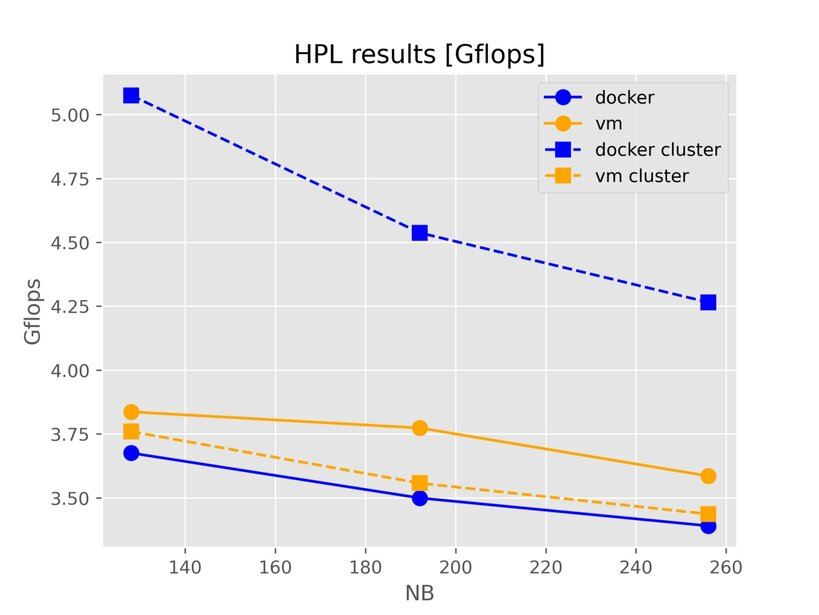
\includegraphics[width=\textwidth]{graphs/HPL_results.jpg}
        \caption{HPL computational results for different architectures and tecnology}
        \label{fig:computational_power_single_nodes}
    \end{subfigure}
    \hfill
    \begin{subfigure}[b]{0.45\textwidth}
        \centering
        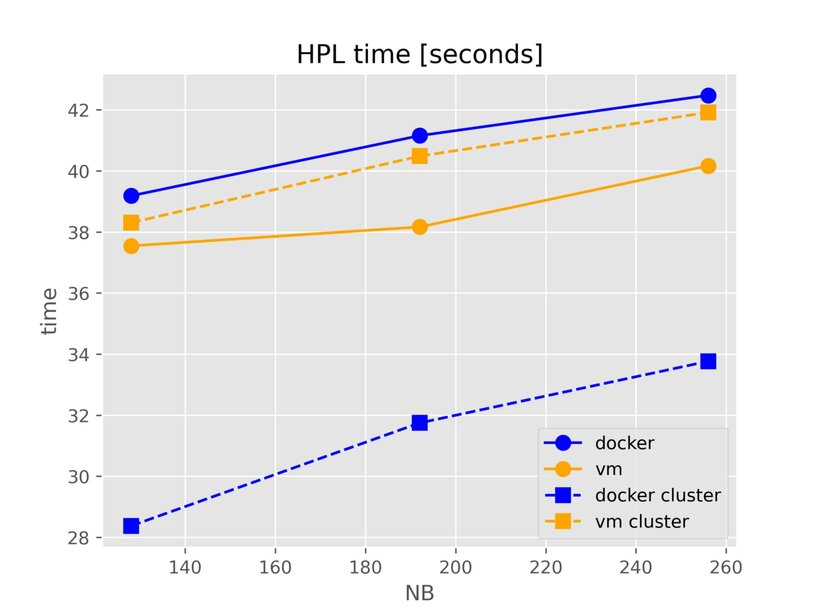
\includegraphics[width=\textwidth]{graphs/HPL_time.jpg}
        \caption{HPL execution times for different architectures and tecnology}
        \label{fig:execution_time_single_nodes}
    \end{subfigure}
    \caption{HPL results that compares single node and cluster for VM and for docker: time (a) and processing power (b).}
    \label{fig:HPL_results_single_nodes}
\end{figure}

We can see the same effect described before in figure \ref{fig:HPL_results_cluster}. Here,  the graph shows the performance of the VM cluster and the Docker cluster, for N=6000 problem and N=10000 problem. For bigger problem,  Docker performs worse than smaller one, while for VM is the opposite.

\begin{figure}[htbp]
    \centering
    \begin{subfigure}[b]{0.45\textwidth}
        \centering
        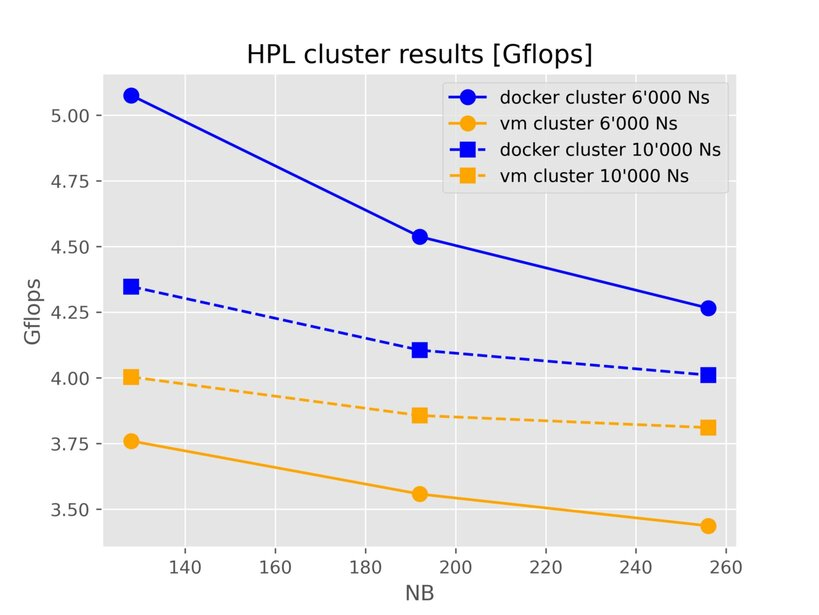
\includegraphics[width=\textwidth]{graphs/HPL_cluster_results.jpg}
        \caption{HPL computational results in a cluster}
        \label{fig:computational_power_cluster}
    \end{subfigure}
    \hfill
    \begin{subfigure}[b]{0.45\textwidth}
        \centering
        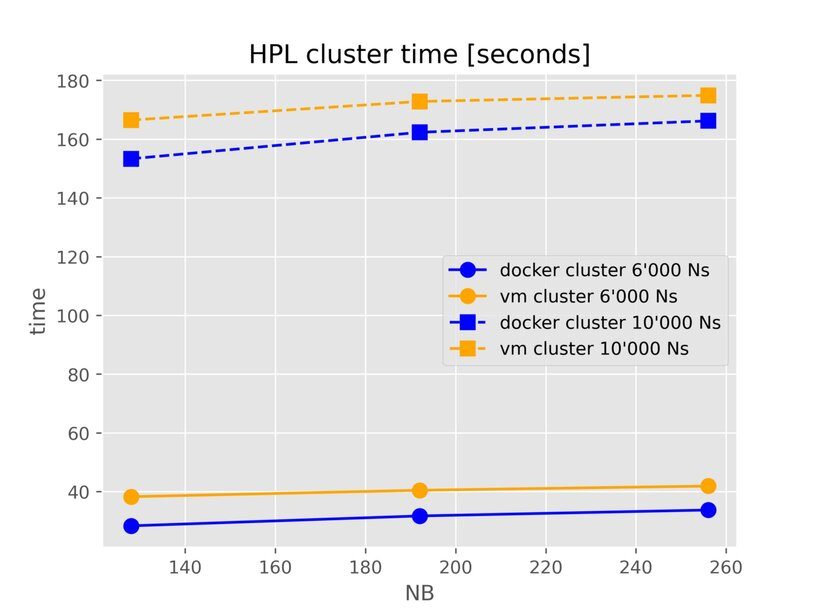
\includegraphics[width=\textwidth]{graphs/HPL_cluster_time.jpg}
        \caption{HPL execution times in a cluster}
        \label{fig:execution_time_cluster}
    \end{subfigure}
    \caption{HPL results for multiple nodes, N=6000 vs N=10000: time (a) and processing power (b).}
    \label{fig:HPL_results_cluster}
\end{figure}

In summary, if the problem is large enough, the cluster always performs better, even if it is implemented with a virtual machine. If the problem is small, the cluster of VM is lacking because of communication overhead. Instead, the VM single core performs better than the Docker single core because the dedicated resources strongly increase the performance. This is a problem, again, just for small problems. For large problems, this problem disappears.

\subsection{FFT}

In this test we can see the same behavior of HPL. Docker cluster performs slightly better than all the other configurations,
while VM single node outperforms Docker single node and VM cluster.

\begin{figure}[htbp] % 'h!' tenta di forzare la posizione "qui"
    \centering
    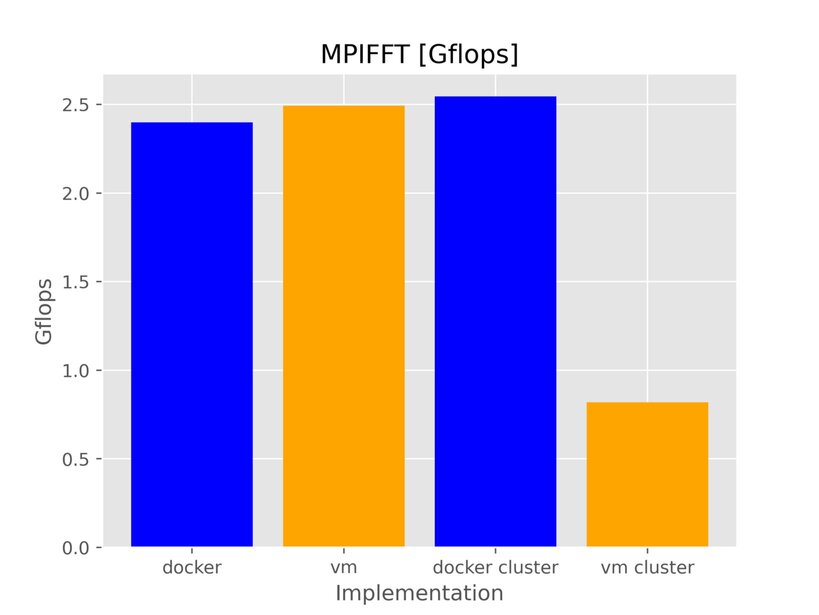
\includegraphics[width=0.8\textwidth]{graphs/MPIFFT.jpg}
    \caption{MPIFFT performance test}
    \label{fig:mpifft}
\end{figure}

The results are shown in Figure \ref{fig:mpifft}. The VM cluster performes more than 60\% less than VM single node. \\
For the other three configurations, the performance is very similar. This should be because FFT test is not as demanding as HPL so the test cannot have a big performance difference.

\subsection{starDGEMM}

This test is very CPU intensive, and the results are really surprising. \\
In Figure \ref{fig:stardgemm}, we can see that the single node configurations perform more than double the cluster configurations.
The answer that I can give is that the moltiplication of matrices was too small to be efficently parallelized.
This leads to a large communication overhead that penalized the cluster configurations.

\begin{figure}[htbp] % 'h!' tenta di forzare la posizione "qui"
    \centering
    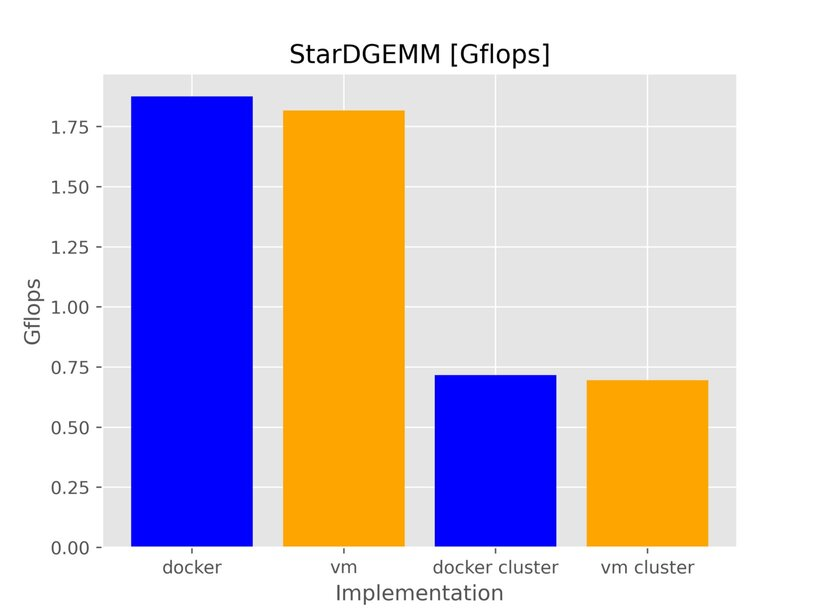
\includegraphics[width=0.8\textwidth]{graphs/StarDGEMM.jpg}
    \caption{StarDGEMM performance test}
    \label{fig:stardgemm}
\end{figure}

\subsection{stress-ng}

In this test we can see that the performance of Docker and VM are very similar.
I run this test for different timeouts (60s, 120s, 180s) and the results are almost the same.
So we can conclude that both technologies are able to provide the same CPU performance for this kind of test and it's not affected by the timeout. \\
A thing to note is that for both technologies, we can see a node that performs more than twice the other two.
I think this effect is due to the CPU architecture and the way the OS allocates the resources.

\begin{figure}[htbp] % 'h!' tenta di forzare la posizione "qui"
    \centering
    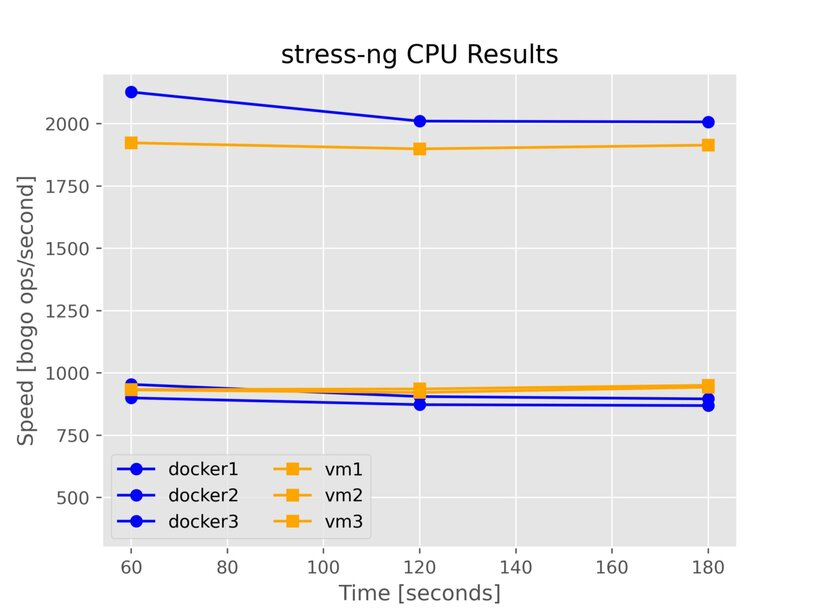
\includegraphics[width=0.8\textwidth]{graphs/stressng_cpu_stress_test.jpg}
    \caption{stress-ng: CPU performance test}
    \label{fig:stress_ng_cpu}
\end{figure}

\subsection{sysbench}

In this test we can see that Docker and VM have almost the same performance.
The results are very similar for all the different \texttt{prime numbers}. \\
This result is reasonable because the allocated resources are the same and in
this case the virtualization overhead is negligible.

\begin{figure}[htbp] % 'h!' tenta di forzare la posizione "qui"
    \centering
    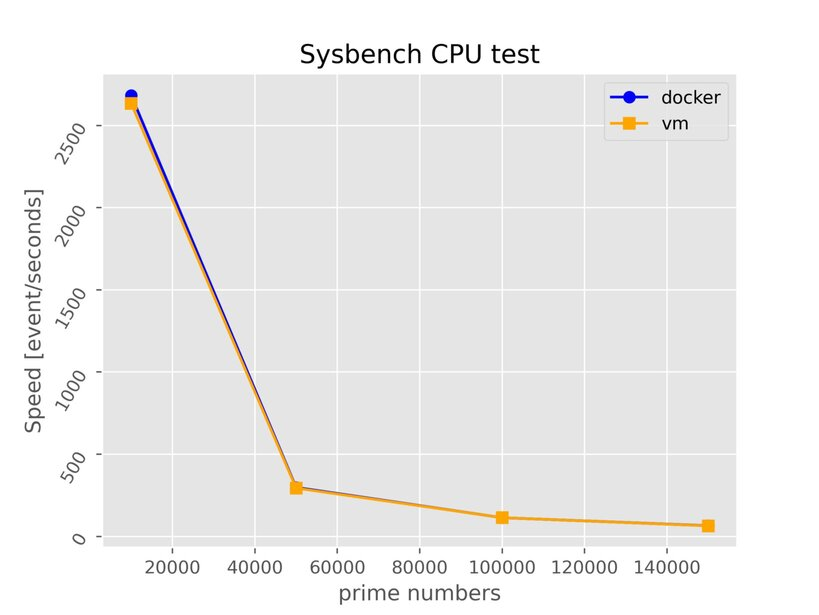
\includegraphics[width=0.8\textwidth]{graphs/sysbench_cpu.jpg}
    \caption{sysbench: CPU performance test}
    \label{fig:sysbench_cpu}
\end{figure}

\section{Results: Memory}

In this section, I analyze the results of the tests that stress memory.
The memory in VM is very different compared to Docker,
because in VM the memory is allocated and dedicated, while in Docker the memory is shared with the host OS. \\
This characteristic theoretically slows down the VM memory performance.

\subsection{MPI random access}

Even in this case we can see the outperformance of single node configurations over cluster ones.
Docker single node performs slightly better than VM single node, while Docker cluster performs better than VM cluster. \\
Obviously, the communication overhead penalizes the cluster configurations.
In a cluster enviroment, the memory access is slower because of the network latency.

\begin{figure}[htbp] % 'h!' tenta di forzare la posizione "qui"
    \centering
    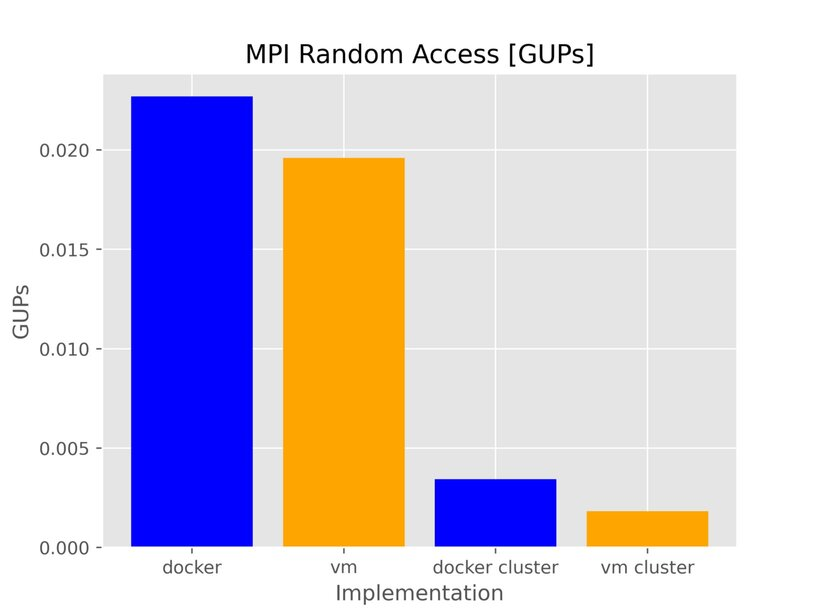
\includegraphics[width=0.8\textwidth]{graphs/MPI_Random_Access.jpg}
    \caption{MPI Random Access performance }
    \label{fig:mpi_random_access}
\end{figure}

\subsection{starSTREAM triad}

We can analyze the same behavior of previous test in Figure \ref{fig:starstream_triad}.
The single node configurations outperform the cluster ones,
and Docker performs slightly better than VM in both configurations. \\
In this test, more than the previous one, the difference between Docker and VM is not so marked.
I think becouse this test is more focused on memory bandwidth rather than latency.

\begin{figure}[htbp] % 'h!' tenta di forzare la posizione "qui"
    \centering
    % Sostituisci 'placeholder.jpg' con il nome del tuo file immagine
    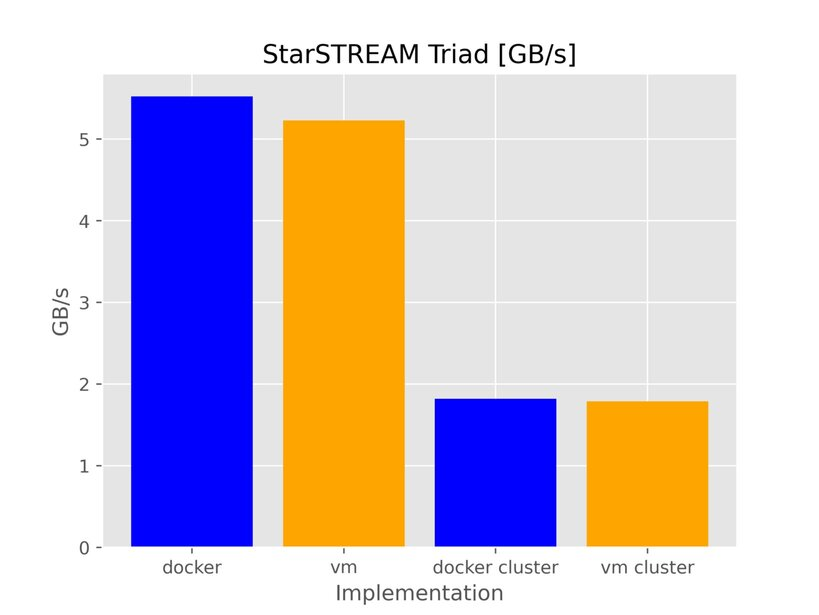
\includegraphics[width=0.8\textwidth]{graphs/StarSTREAM_Triad.jpg}
    \caption{StarSTREAM Triad performance}
    \label{fig:starstream_triad}
\end{figure}

\subsection{stress-ng}

\begin{figure}[htbp] % 'h!' tenta di forzare la posizione "qui"
    \centering
    % Sostituisci 'placeholder.jpg' con il nome del tuo file immagine
    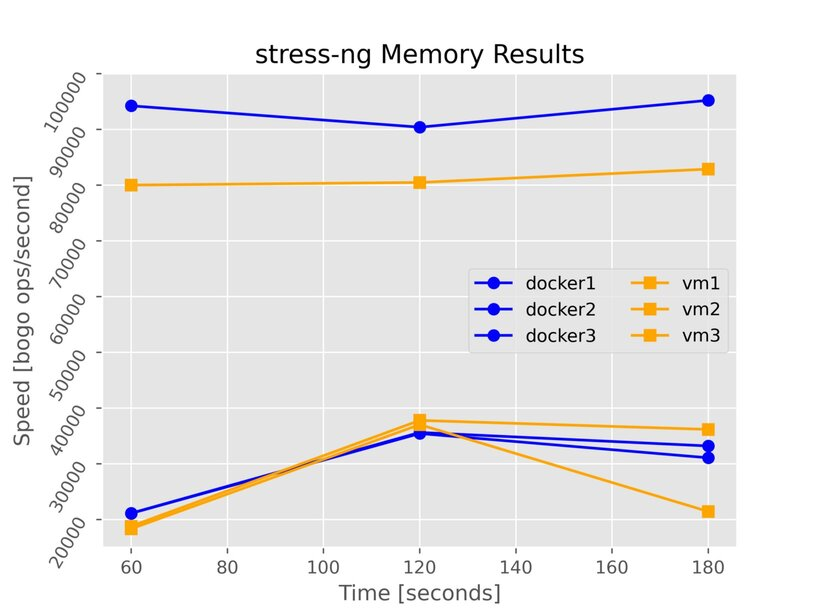
\includegraphics[width=0.8\textwidth]{graphs/stressng_memory_stress_test.jpg}
    \caption{stress-ng memory test performance}
    \label{fig:stress-ng_memory}
\end{figure}

In this test, that is the memory version of stress-ng, we can see a similar behavior of the CPU version.
Docker has better performance than VM almost always. \\
All the considerations made for the CPU version about cores are valid also for this memory version.

\subsection{sysbench}

This test are the same of the CPU version, but focused on memory, but the results are very different. \\
The performance of Docker is noticeably better than VM. This is because the memory allocation in VM is dedicated and fixed,
while in Docker the memory is shared with the host OS, making the access faster. \\
I need to repeat this test for different \texttt{memory sizes} to see when the data became stable, with no more big changes.

\begin{figure}[htbp] % 'h!' tenta di forzare la posizione "qui"
    \centering
    % Sostituisci 'placeholder.jpg' con il nome del tuo file immagine
    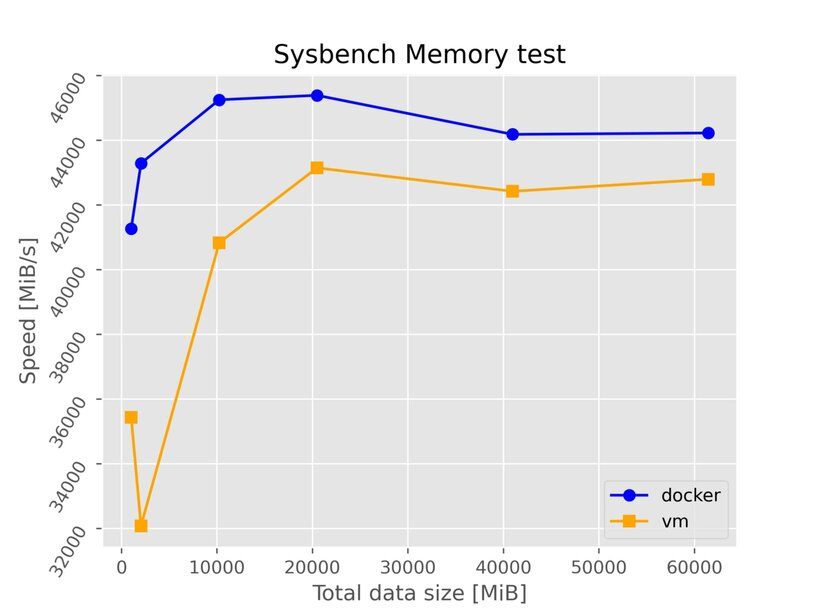
\includegraphics[width=0.8\textwidth]{graphs/sysbench_memory.jpg}
    \caption{sysbench memory test performance}
    \label{fig:sysbench_memory}
\end{figure}

\section{Results: Disk}

In this section I will analyze the results of the disk performance tests. \\
For disk performance test, the main tool used is iozone. I decide to test with and without direct I/O,
that is a way to bypass the cache and write/read directly on the disk. \\
In this way it emerges how the caching system can influence the performances.

\subsection{iozone: no direct I/O}

I start with the results without direct I/O, so with caching system enabled.
I tested both in local directory and shared directory. \\
Theoretically, the shared directory is slower because of the network overhead.

\begin{figure}[htbp]
    \centering
    % --- Prima Immagine ---
    \begin{subfigure}[b]{0.45\textwidth}
        \centering
        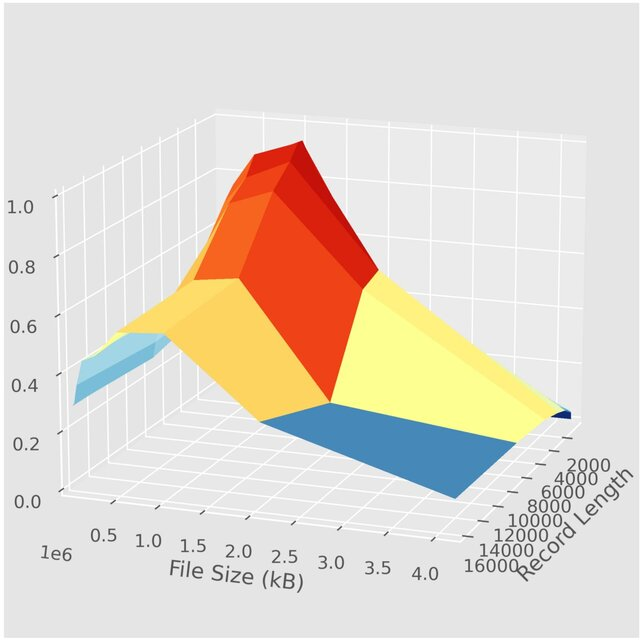
\includegraphics[width=\textwidth]{graphs/docker_iozone_locale_cache_rread_3d_plot.jpg}
    \end{subfigure}
    \hfill % Questo comando spinge le immagini ai bordi opposti
    % --- Seconda Immagine ---
    \begin{subfigure}[b]{0.45\textwidth}
        \centering
        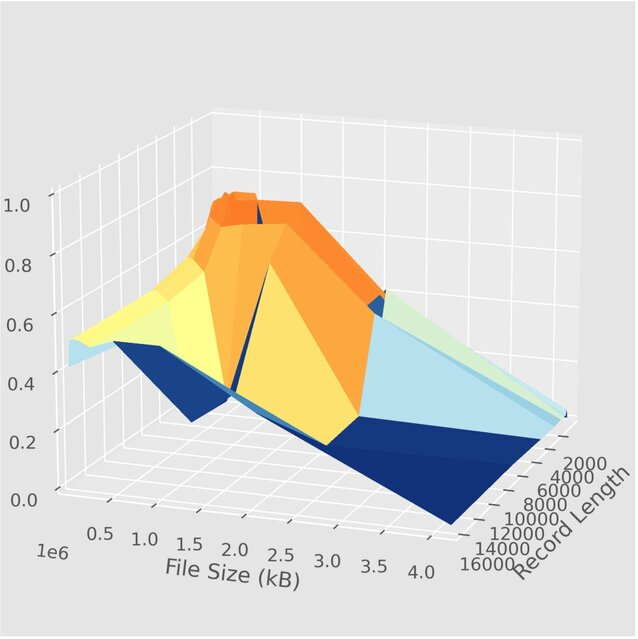
\includegraphics[width=\textwidth]{graphs/docker_iozone_locale_cache_rwrite_3d_plot.jpg}
    \end{subfigure}
    \vfill
    \begin{subfigure}[b]{0.45\textwidth}
        \centering
        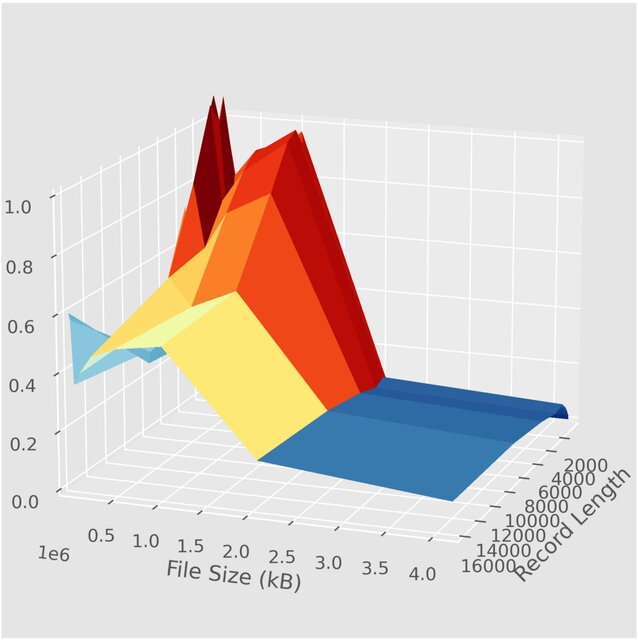
\includegraphics[width=\textwidth]{graphs/vm_iozone_locale_cache_rread_3d_plot.jpg}
    \end{subfigure}
    \hfill
    \begin{subfigure}[b]{0.45\textwidth}
        \centering
        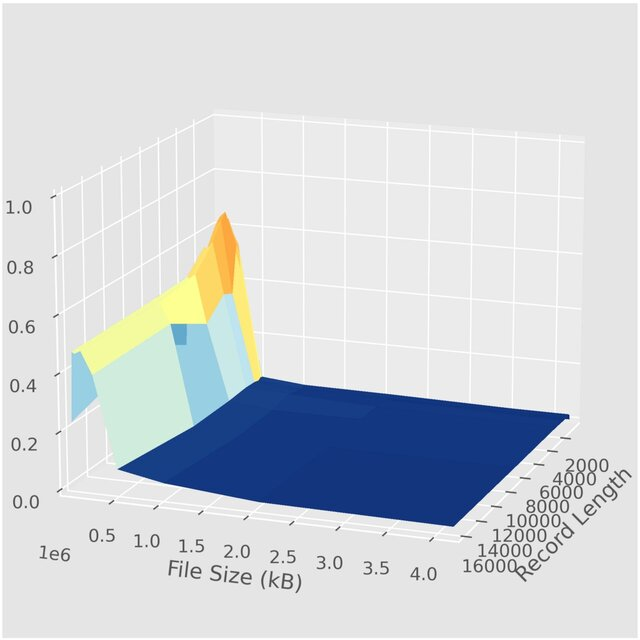
\includegraphics[width=\textwidth]{graphs/vm_iozone_locale_cache_rwrite_3d_plot.jpg}
    \end{subfigure}
    % --- Didascalia Generale ---
    \caption{iozone local directory performance with no direct I/O: (a) random read (docker), (b) random write (docker), (c) random read (vm) (d) random write (vm)}
    \label{fig:iozone_no_direct_io}
\end{figure}

In figure \ref{fig:iozone_no_direct_io} we have four plots:
in the left side the docker results, in the right side the VM results,
in the first row the random read results, in the second row the random write results. \\
It is clear that Docker performs decisively better than VM in both read and write operations.
This effect is due to the fact that VM use a virtualized disk that slow down the operations. \\
I suppose that, with caching system enabled, the difference is more marked because the cache system is more efficient in Docker than in VM.

\begin{figure}[htbp]
    \centering
    % --- Prima Immagine ---
    \begin{subfigure}[b]{0.45\textwidth}
        \centering
        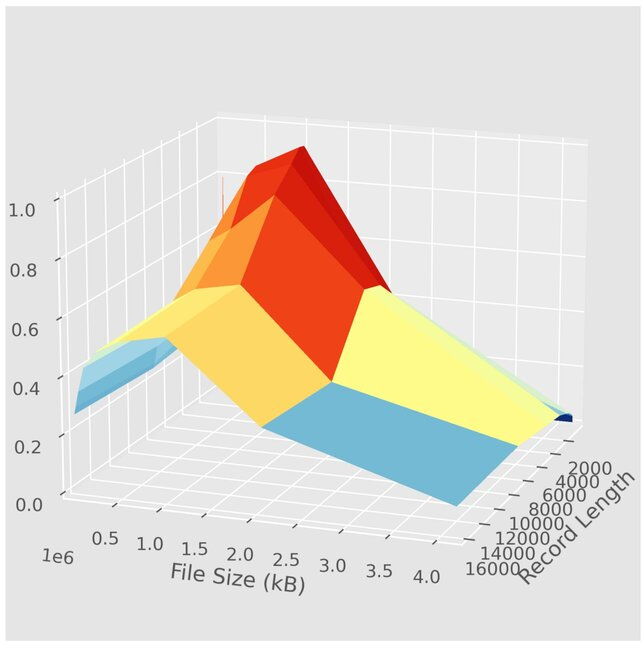
\includegraphics[width=\textwidth]{graphs/docker_iozone_condivisa_cache_rread_3d_plot.jpg}
    \end{subfigure}
    \hfill % Questo comando spinge le immagini ai bordi opposti
    % --- Seconda Immagine ---
    \begin{subfigure}[b]{0.45\textwidth}
        \centering
        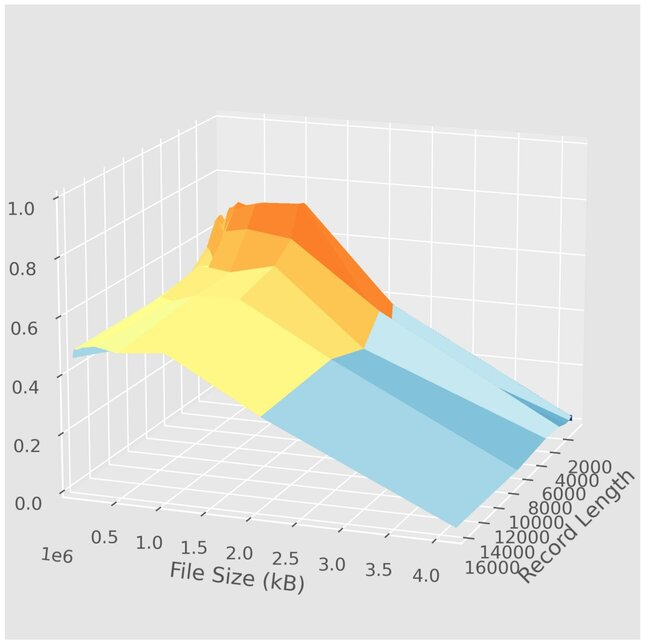
\includegraphics[width=\textwidth]{graphs/docker_iozone_condivisa_cache_rwrite_3d_plot.jpg}
    \end{subfigure}
    \vfill
    \begin{subfigure}[b]{0.45\textwidth}
        \centering
        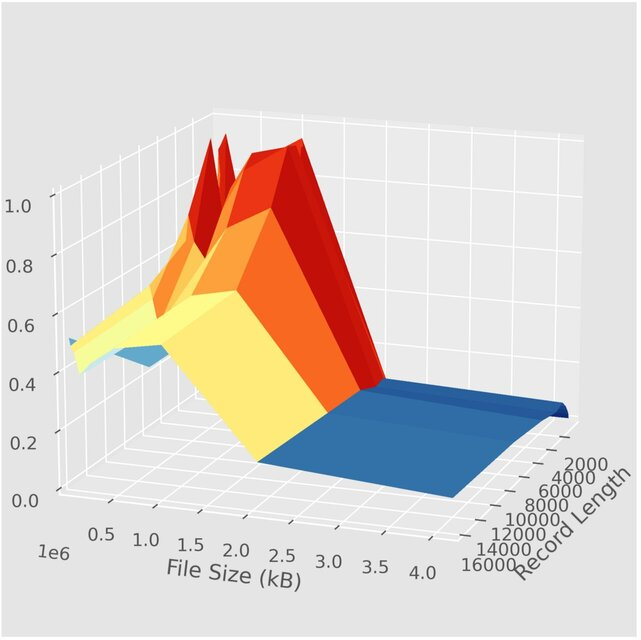
\includegraphics[width=\textwidth]{graphs/vm_iozone_condivisa_cache_rread_3d_plot.jpg}
    \end{subfigure}
    \hfill
    \begin{subfigure}[b]{0.45\textwidth}
        \centering
        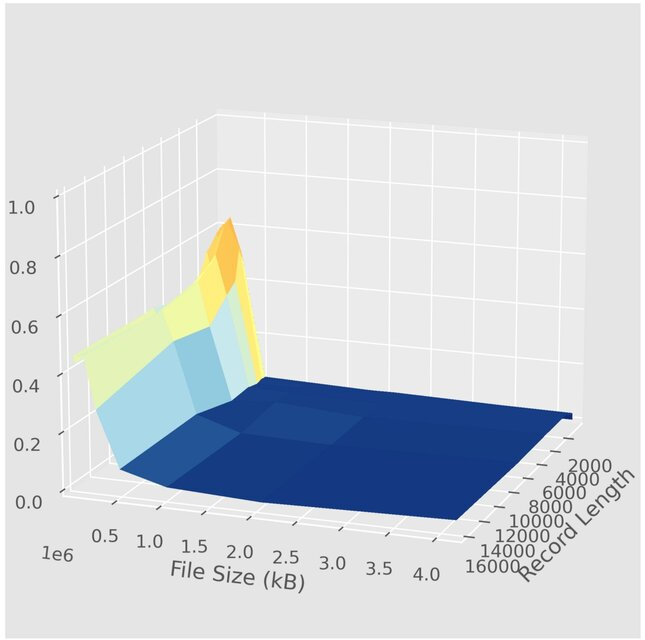
\includegraphics[width=\textwidth]{graphs/vm_iozone_condivisa_cache_rwrite_3d_plot.jpg}
    \end{subfigure}
    % --- Didascalia Generale ---
    \caption{iozone shared directory performance with no direct I/O: (a) random read (docker), (b) random write (docker), (c) random read (vm) (d) random write (vm)}
    \label{fig:iozone_no_direct_io_shared}
\end{figure}

In the shared directory case, shown in figure \ref{fig:iozone_no_direct_io_shared}, the results are overall similar. \\
The differences, compared to local test, are negligible.

\subsection{iozone: direct I/O}

Iozone test with direct I/O, so without caching system, gives us interesting results.
First of all, I set the same scale as the previous test to have a better comparison. \\
The results, shown in figure \ref{fig:iozone_direct_io}, are really different from the previous test. \\
The similarities between the four previous plots are that Docker always performs better than VM. \\
The graphs show a decrease in performance of about one order of magnitude compared to the previous test with caching system.
This prove us how important is the caching system for disk performance. \\
In a qualitative way, not quantitative, the behavior is similar to the previous test.

\begin{figure}[htbp]
    \centering
    % --- Prima Immagine ---
    \begin{subfigure}[b]{0.45\textwidth}
        \centering
        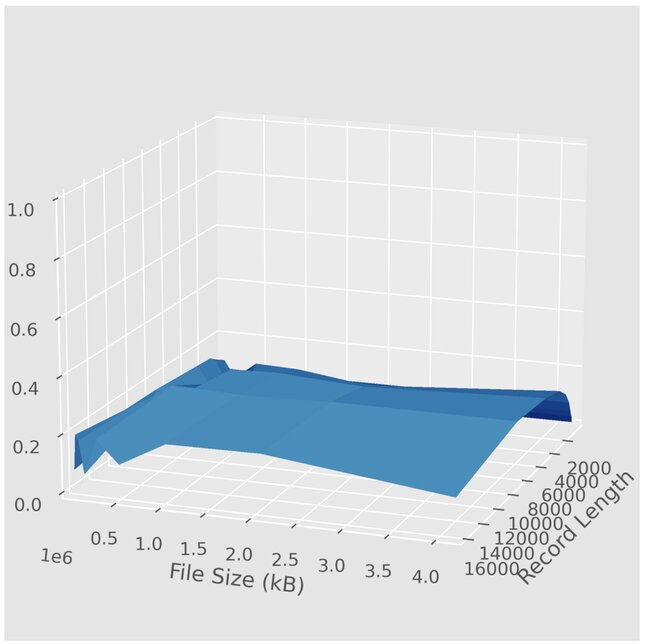
\includegraphics[width=\textwidth]{graphs/docker_iozone_locale_no_cache_rread_3d_plot.jpg}
    \end{subfigure}
    \hfill % Questo comando spinge le immagini ai bordi opposti
    % --- Seconda Immagine ---
    \begin{subfigure}[b]{0.45\textwidth}
        \centering
        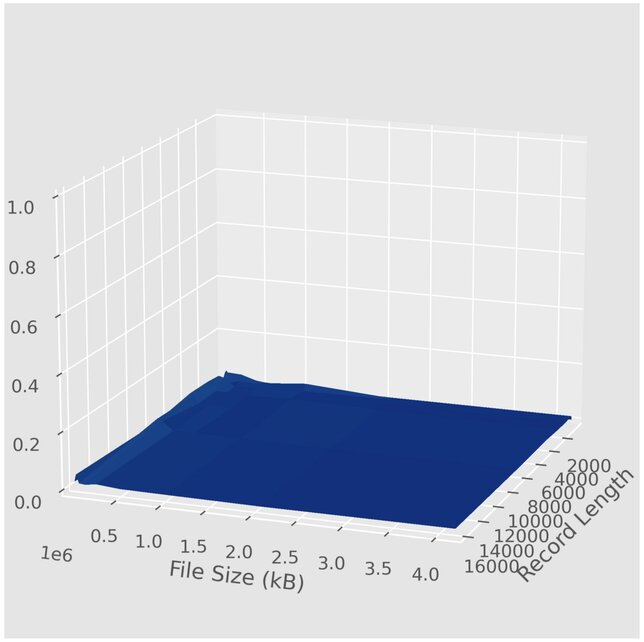
\includegraphics[width=\textwidth]{graphs/docker_iozone_locale_no_cache_rwrite_3d_plot.jpg}
    \end{subfigure}
    \vfill
    \begin{subfigure}[b]{0.45\textwidth}
        \centering
        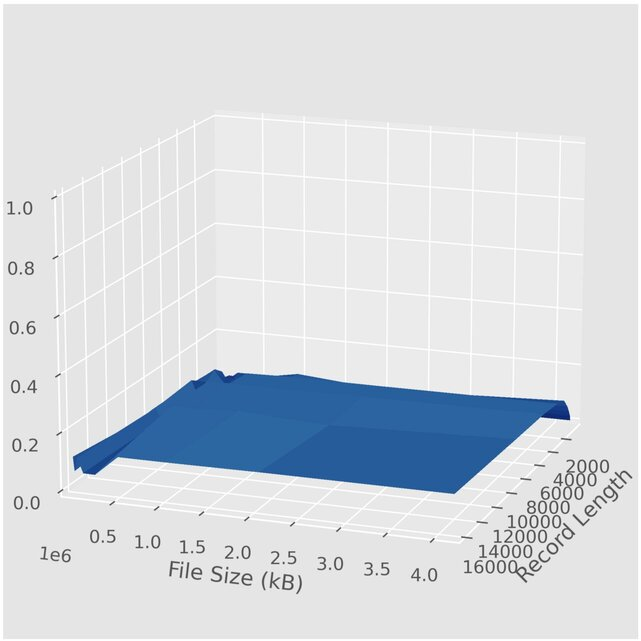
\includegraphics[width=\textwidth]{graphs/vm_iozone_locale_no_cache_rread_3d_plot.jpg}
    \end{subfigure}
    \hfill
    \begin{subfigure}[b]{0.45\textwidth}
        \centering
        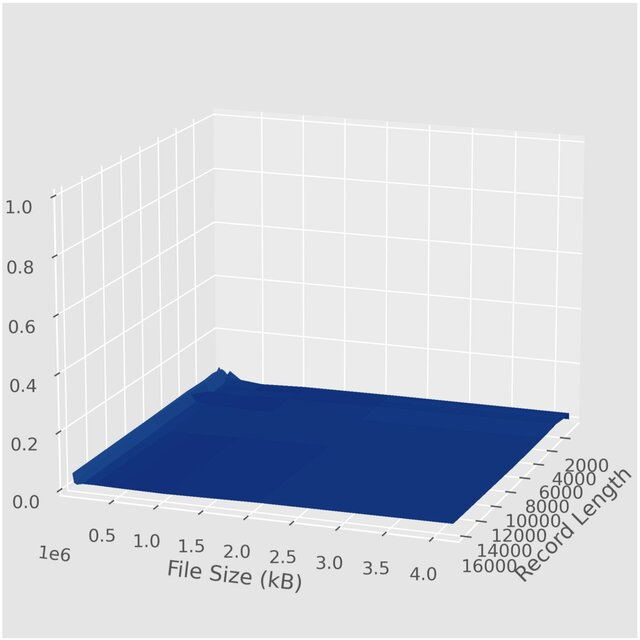
\includegraphics[width=\textwidth]{graphs/vm_iozone_locale_no_cache_rwrite_3d_plot.jpg}
    \end{subfigure}
    % --- Didascalia Generale ---
    \caption{iozone local directory performance with direct I/O: (a) random read (docker), (b) random write (docker), (c) random read (vm) (d) random write (vm)}
    \label{fig:iozone_direct_io}
\end{figure}

In figure \ref{fig:iozone_direct_io_shared}, the results are practically identical both in qualitative and quantitative way. \\
The network overhead does not influence so much the performances in this case. \\
At the end, we can conclude that Docker has better disk performance than VM,
and this because the \textbf{hypervisor} layer in VM slow down the disk operations.

\begin{figure}[htbp]
    \centering
    % --- Prima Immagine ---
    \begin{subfigure}[b]{0.45\textwidth}
        \centering
        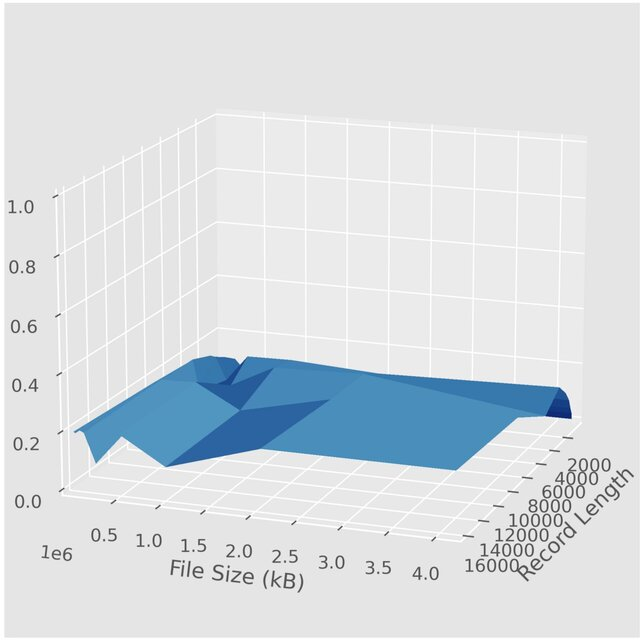
\includegraphics[width=\textwidth]{graphs/docker_iozone_condivisa_no_cache_rread_3d_plot.jpg}
    \end{subfigure}
    \hfill % Questo comando spinge le immagini ai bordi opposti
    % --- Seconda Immagine ---
    \begin{subfigure}[b]{0.45\textwidth}
        \centering
        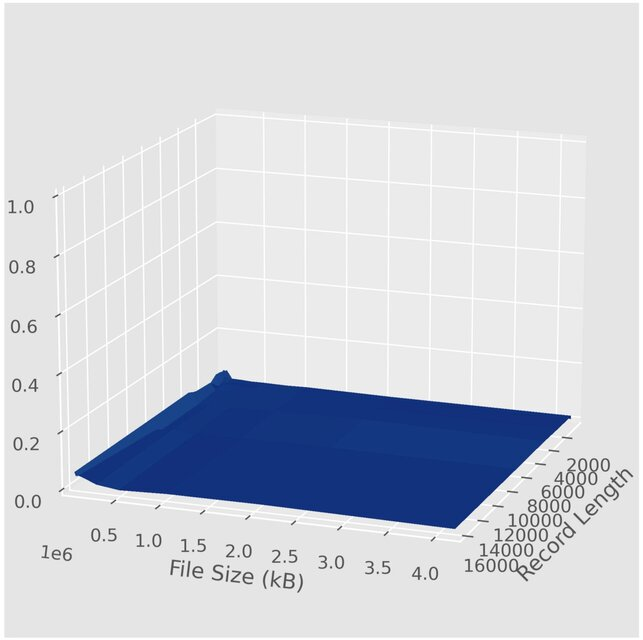
\includegraphics[width=\textwidth]{graphs/docker_iozone_condivisa_no_cache_rwrite_3d_plot.jpg}
    \end{subfigure}
    \vfill
    \begin{subfigure}[b]{0.45\textwidth}
        \centering
        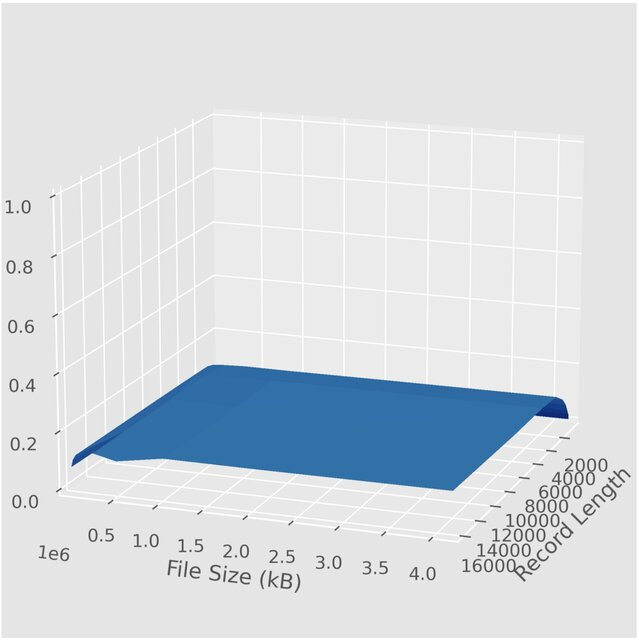
\includegraphics[width=\textwidth]{graphs/vm_iozone_condivisa_no_cache_rread_3d_plot.jpg}
    \end{subfigure}
    \hfill
    \begin{subfigure}[b]{0.45\textwidth}
        \centering
        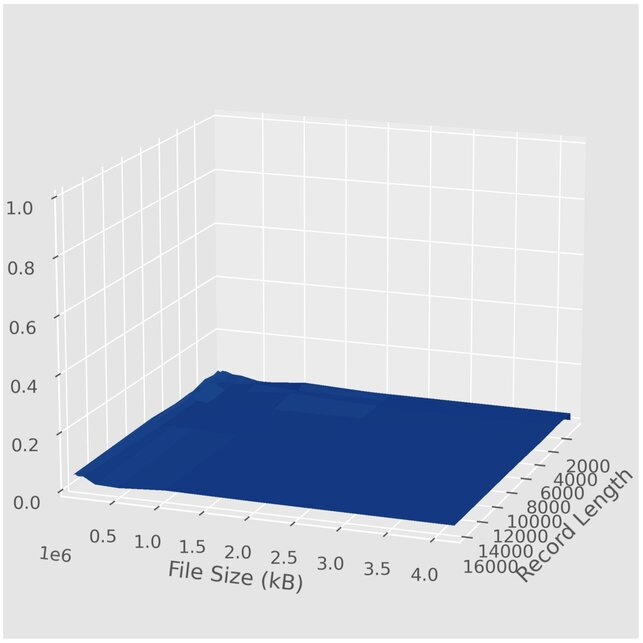
\includegraphics[width=\textwidth]{graphs/vm_iozone_condivisa_no_cache_rwrite_3d_plot.jpg}
    \end{subfigure}
    % --- Didascalia Generale ---
    \caption{iozone shared directory performance with direct I/O: (a) random read (docker), (b) random write (docker), (c) random read (vm) (d) random write (vm)}
    \label{fig:iozone_direct_io_shared}
\end{figure}

\section{Results: Communication}
\subsection{iperf3}

As last test, I analyze the network communication performance with iperf3.
The result, shown in figure \ref{fig:iperf3}, does not leave space for doubts. \\
Docker outperforms VMs by a large margin. This is because the network virtualization in VM
adds a large overhead that strongly penalizes the communication performance.

\begin{figure}[htbp] % 'h!' tenta di forzare la posizione "qui"
    \centering
    % Sostituisci 'placeholder.jpg' con il nome del tuo file immagine
    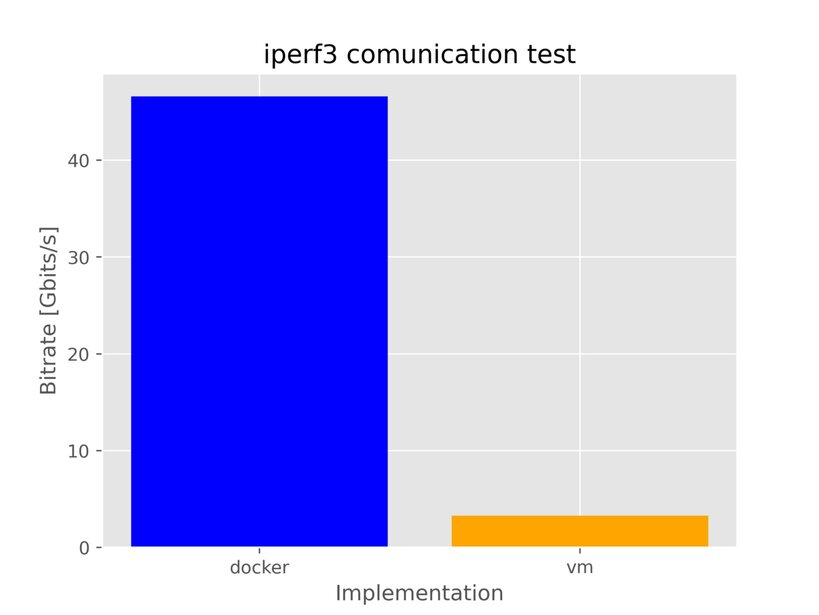
\includegraphics[width=0.8\textwidth]{graphs/iperf3.jpg}
    \caption{iperf3 comunication performance}
    \label{fig:iperf3}
\end{figure}

The difference is more than an order of magnitude,
making Docker in strong advantage for network communication services. \\
The test was done using TCP protocol, that is the most used in network communication. \\
The two involved nodes are in the same physical machine, so the results should be even more marked. \\
In the previous tests, often the explanation of the difference between Docker and VM could be attributed to the inefficient communication between nodes in VM. \\
Here, this effect is evident and quantifiable.

\chapter{Conclusions}

In this report, we have explored the fundamental concepts and practical applications of VM and Docker containerization technology.
I began by discussing the architecture of Virtual Machines (VMs) and I then examined the process of creating and managing VMs,
highlighting best practices for optimizing performance and security.
I then briefly discussed Docker, including its components such as Docker Engine, Docker Images, and Docker Containers.
I then delved into the process of creating and managing Docker images, highlighting best practices for building efficient and secure images. \\
Finally, I compared VMs and Docker containers, discussing their respective advantages and disadvantages,
and provided guidance on when to use each technology based on specific use cases and requirements. \\
Overall, this report told that both VMs and Docker containers are powerful tools for managing and deploying applications,
but the performance and efficiency of Docker containers make them a more attractive option for many use cases. \\
Personally, I found Docker even easier to use and manage compared to VMs. The program installation and configuration process was straightforward,
the rapidity of deployment was impressive, and the portability in other systems made it a versatile choice for various applications. \\
Nonetheless, VMs still have their place in certain scenarios, such as when running legacy applications or when a higher level of isolation is required. \\
In conclusion, the choice between VMs and Docker containers ultimately depends on the specific needs and requirements of the application being deployed,
but it is comprehensible that containerization technology is becoming increasingly popular in modern software development and deployment practices.

\clearpage

\end{document}